\section{Design di dettaglio}

Dopo aver descritto l’architettura del sistema si procede con il design di dettaglio delle sue componenti principali. 
L’approccio progettuale utilizzato combina aspetti Object-oriented, come l’utilizzo dell’interfaccia come astrazione attraverso la quale caratterizzare i componenti, per scatenare comportamenti diversi su entità soggette ad un comune contratto, con elementi di programmazione funzionale pura, quali la tendenza all’impiego di strutture dati immutabili e la riduzione di side effects, favorendo la descrizione lazy della computazione, la separazione fra componente strutturale e comportamentale delle entità ed altri elencati di seguito.


\subsection{Core}
ciao


\begin{figure}[h!]
\centering
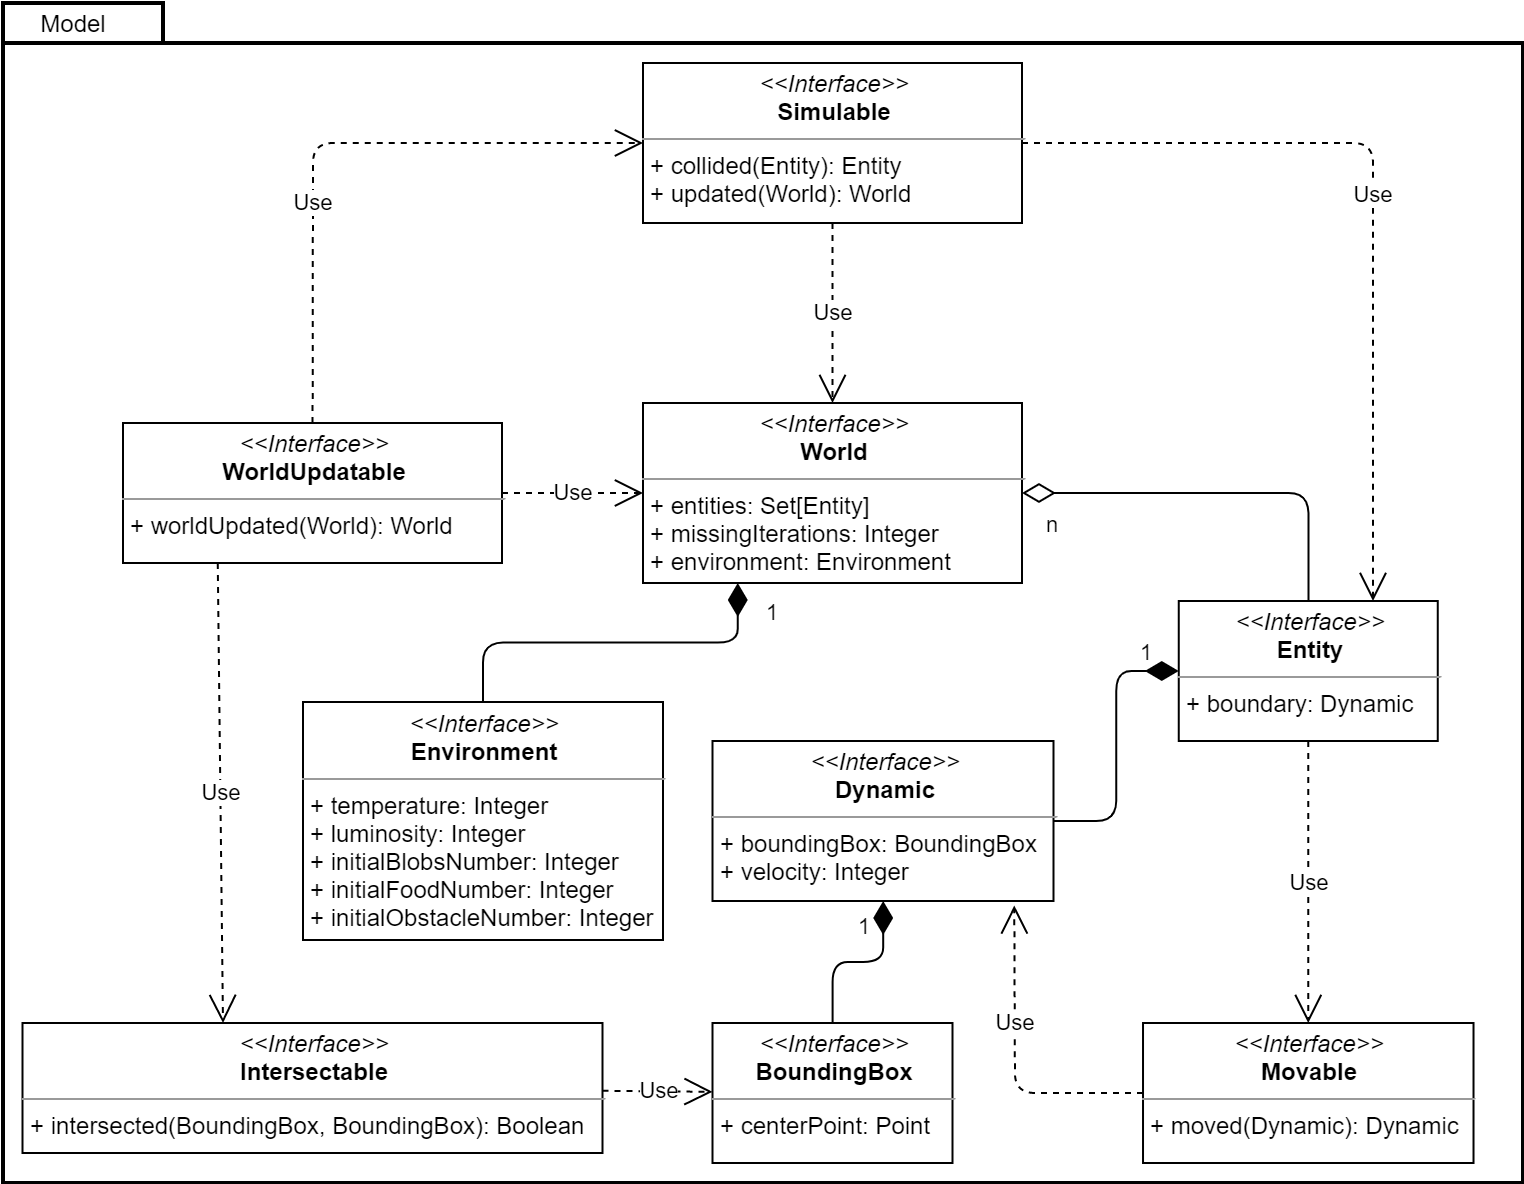
\includegraphics[width=\textwidth, scale=0.44]{img/Model.png}
\caption{Design Model}
\label{fig:model}
\end{figure}

\begin{figure}[h!]
\centering
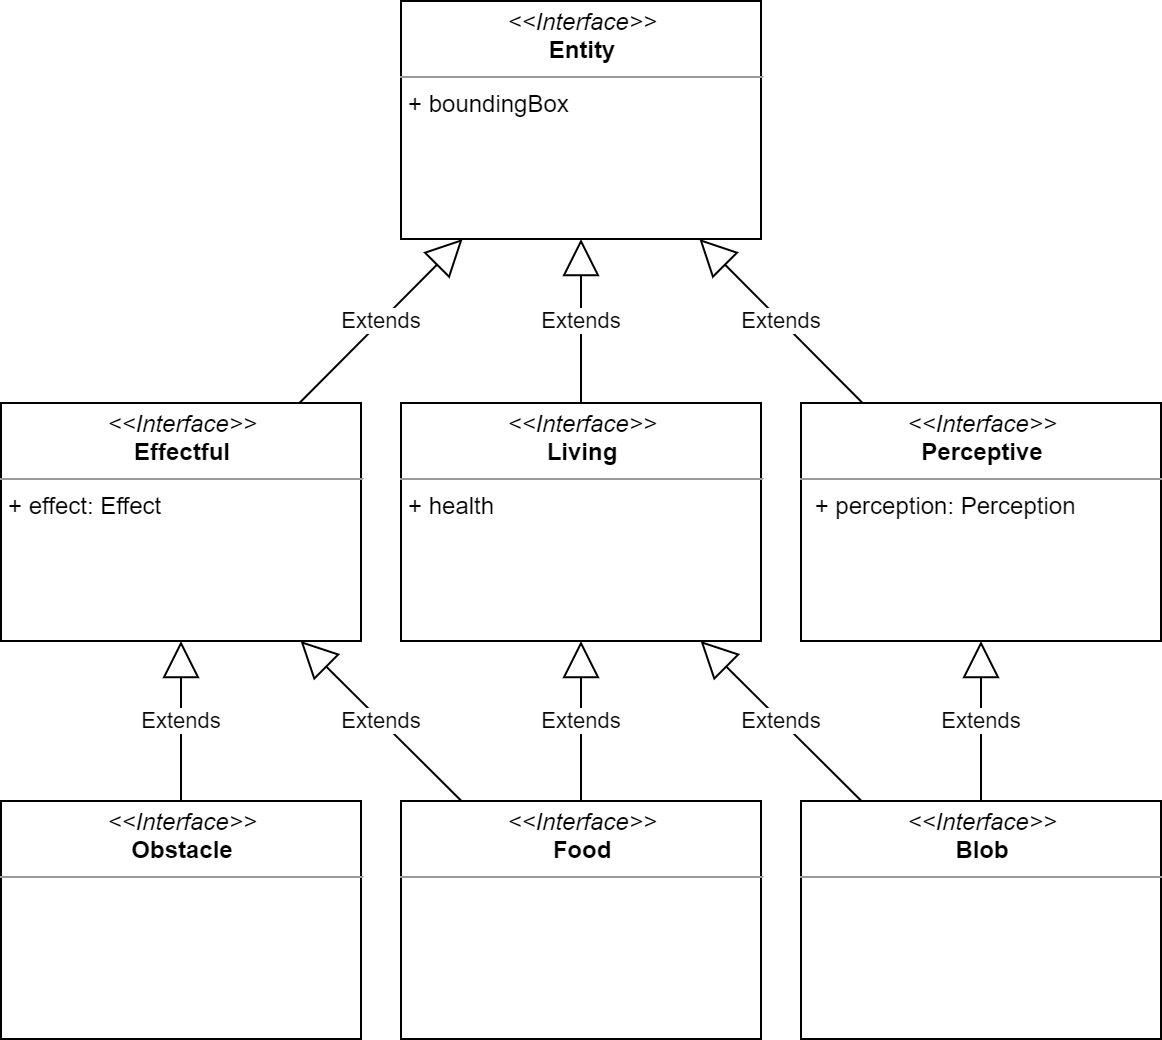
\includegraphics[width=\textwidth, scale=0.44]{img/ModelHierarchy.png}
\caption{Gerarchia Model}
\label{fig:modelhierarchy}
\end{figure}